%Quark Matter 2014 poster - 

\documentclass[final]{beamer}
\usepackage[orientation=portrait,size=a0,
            scale=1.3     % font scale factor
           ]{beamerposter}

\newcommand{\nn}{\nonumber \\}
\newcommand{\pt}{$p_{T}$}
\newcommand{\jw}{\textsc{Jewel}~}
\newcommand{\jwpy}{\textsc{Jewel+Pythia}~}
\newcommand{\py}{\textsc{Pythia}~}


           
\geometry{
  hmargin=2cm, % little modification of margins
}
\setbeamertemplate{itemize/enumarate body begin}{\tiny}
%\setbeamertemplate{itemize/enumerate sub body begin}{\tiny}
%
\usepackage[utf8]{inputenc}

\linespread{1}
%
%==The poster style============================================================
\usetheme{sharelatex}

%==Title, date and authors of the poster=======================================
\title
[Quark Matter 2018] % Conference
{ % Poster title
Quark and Gluon Jet SubStructure  \\ in Heavy Ion Collisions - arXiv:1803.03589 
}

\author{Yang-Ting Chien $^{a}$ and Raghav Kunnawalkam Elayavalli $^{b}$\\
{\normalsize $^{a}$ Center for Theoretical Physics, Massachusetts Institute of Technology, Cambridge, MA 02139}\\
{\normalsize $^{b}$ Department of Physics and Astronomy, Wayne State University, Detroit, MI 48201}
%$^{c}$ Department of Physics and Astronomy\\
%$~$ Rutgers, the State University of New Jersey, New Brunswick, NJ 08901
}

\date{\today}

\begin{document}
\begin{frame}[t]

%\section{Abstract}
%We study the phenomenon of jet quenching utilizing quark and gluon jet substructures as independent probes of heavy ion collisions. We exploit jet and subjet features to highlight differences between quark and gluon jets in vacuum and in a medium with the jet-quenching model implemented in \textsc{Jewel}. We begin with a physics-motivated, multivariate analysis of jet substructure observables including the jet mass, the radial moments, the $p_T^D$ and the pixel multiplicity. In comparison, we employ state-of-the-art image-recognition techniques by training a deep convolutional neutral network on jet images. To systematically extract jet substructure information, we introduce the telescoping deconstruction framework exploiting subjet kinematics at multiple angular scales. We draw connections to the soft-drop subjet distribution and illuminate medium-induced jet modifications using Lund diagrams. We find that the quark gluon discrimination performance worsens in heavy ion jets due to significant soft event activity affecting the soft jet substructure. Our work suggests a systematically improvable framework for studying modifications to quark and gluon jet substructures and facilitating direct comparisons between theoretical calculations, simulations and measurements in heavy ion collisions.

%==============================================================================
\begin{multicols}{3}

%==============================================================================
%==The poster content==========================================================
%==============================================================================

\section{Quark and Gluon Jets}

	We systematically study the tagging of quark and gluon jets in both proton-proton and lead-lead collisions making full use of their substructure. Such a complimentary approach studies the differences in the modification of quark v.s. gluon jets, thus disentangling modifications of their common features. 

	\begin{figure}[h]
	  \centering
	  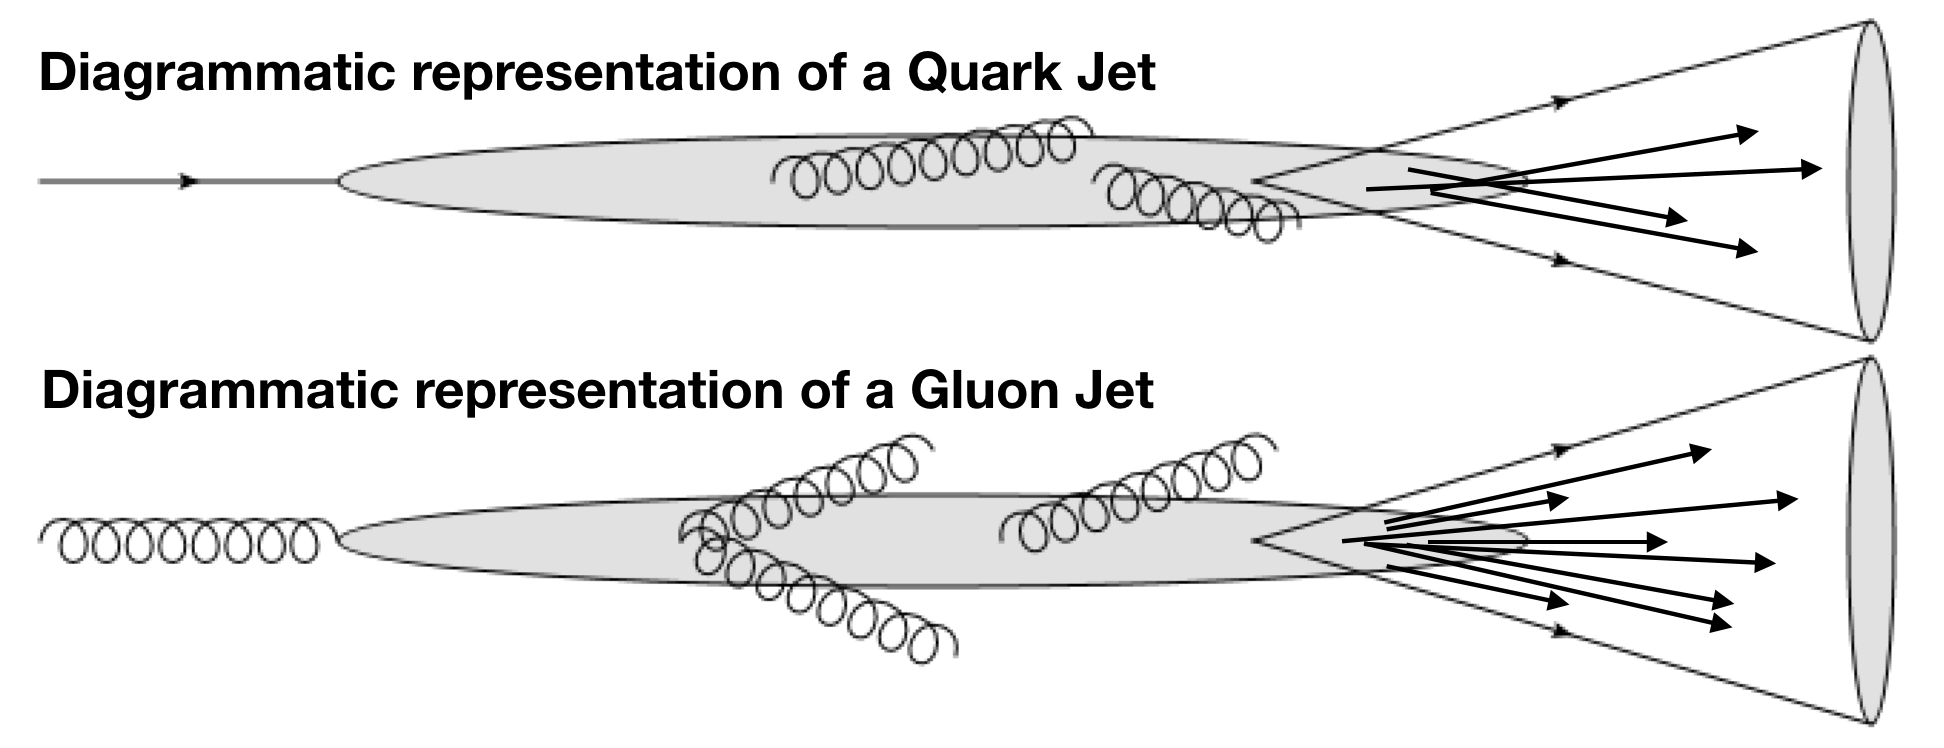
\includegraphics[width=0.9\columnwidth]{Figures/q_g_jet_quenching}
	  \label{fig:qgjetdrawing}
	\end{figure}
	
	At lowest-order, quark and gluon are defined by their jet-initiating partons. Primary differences are 
	\begin{itemize}
	\item The Casimir factors of quark jets and gluon jets are $C_F = 4/3$ and $C_A=3$ 
	\item larger color charge of gluons is expected to result in broader spread of the radiation inside such jets. 
	\end{itemize} 
	
	\subsection{Analysis Details}	
	
	We use the \jw MC heavy ion simulation to produce separate samples of $\gamma+q$ and $\gamma+g$ jet for pp and PbPb (0-20\%) central events at 2.76 TeV. 
	\begin{itemize}
	\item anti-$k_t, R = 0.4$ Jets
	\item $ p^{\gamma}_T > 100~{\rm GeV}, ~|\eta^{\rm \gamma}|<1.5$
	\item $p^{\rm jet}_T > 50~{\rm GeV}, ~ |\eta^{\rm jet}|<1.5, ~\Delta \phi_{\gamma, {\rm jet}} > 2\pi/3 $
	\end{itemize} 
	
\section{Representing Jets}

	We look at two of the different representations of the jet collections in this analysis. 
	
	\begin{itemize}
	\item {\color{green} Physics motivated observables} designed to highlight differences between quark and gluon jets  
		\begin{itemize}
		\item Jet mass and $p_{T}^{D}$
	        \item First radial moment and 0.5 radial moment
       		\item Pixel multiplicity: the number of $(\eta,\phi)$ pixels with nonzero energy deposit.
		\end{itemize}
	\end{itemize}
			
	\begin{figure}[h]
	  \centering
	  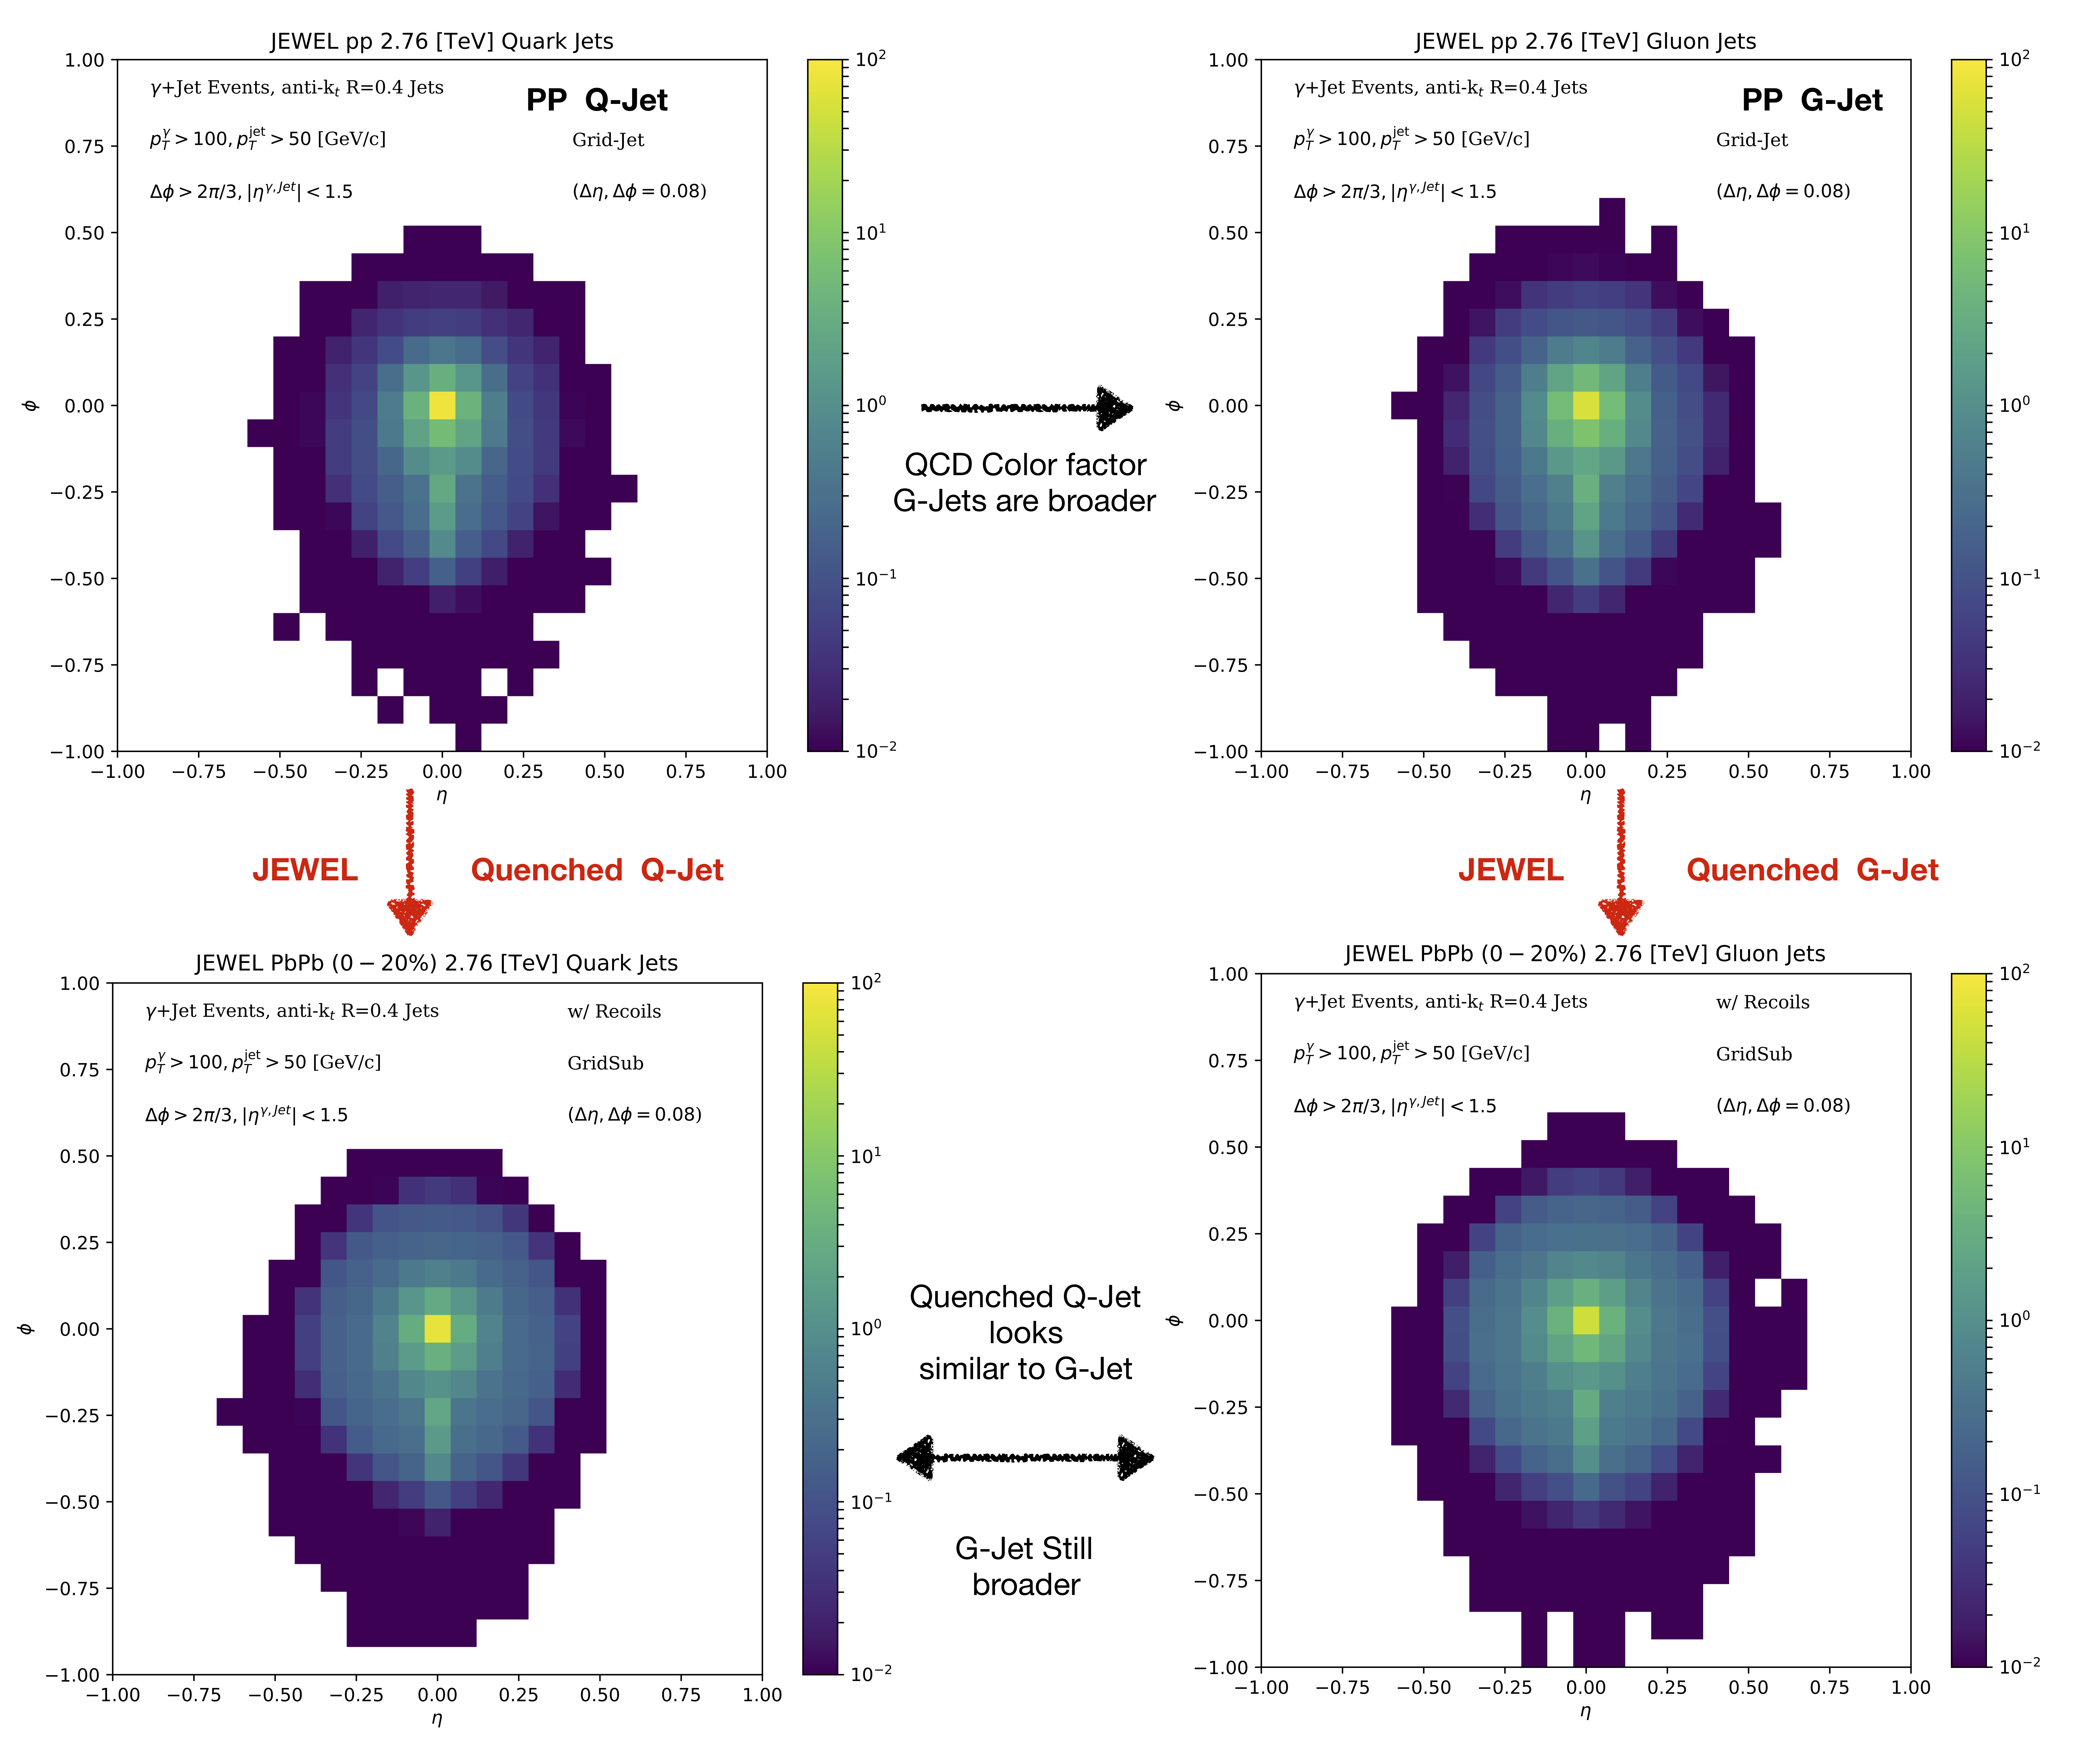
\includegraphics[width=0.9\columnwidth]{Figures/Jet_Image_Quenching_png}
	  \label{fig:qgjetimages}
	\end{figure}

	\begin{itemize}		
	\item {\color{blue} Jet Images} as a fixed-dimensional representation of jet energy distribution in the $\eta-\phi$ plane. 
		\begin{itemize}
			\item Leading jet constituent fixed at (0,0)
			\item Rotated to keep energy flow at 6 o'clock angle.  
		\end{itemize}
	\end{itemize}

	
	\begin{figure}[h]
	  \centering
	  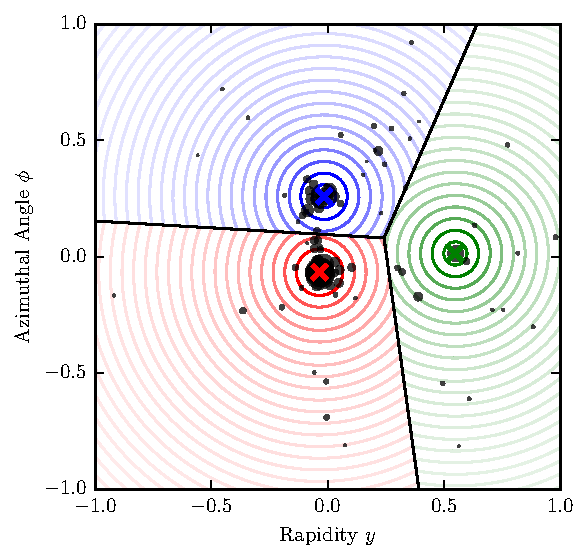
\includegraphics[width=0.8\columnwidth]{Figures/Telescoping.pdf}
	  \label{fig:tjetQCD}
	\end{figure}
	
	\begin{itemize}
	\item {\color{red} Telescoping Deconstruction} (TD) aims to embrace both advantages of multivariate analysis and jet image recognition. 
	\begin{itemize}
	\item It is a complete and systematic expansion of subjet $p_T$ and mass
	\item Expansion is ordered by $N$, the number of subjets exclusively reconstructed
	\item TD provides access to the fragmentation basis of the jet sub-structure
	\end{itemize}
	\end{itemize}
	
\subsection{Machine Learning Tools}
We use neural network models as implemented in Keras with TensorFlow backend. 
	\begin{itemize}
	\item Phys-Vars and TD - MultiLayer Perceptrons (MLP) models with a variety of hidden dense layers and nodes.  
	\item Jet Images - Deep Convolutional Neural Network (DCNN) with three convolution layers of sequentially reducing sizes, each with 8 filters followed by a max-pooling and dense layers w/ dropouts. 
	\end{itemize}
	We perform cross validation using Monte Carlo samples which are split into two random halves for training and testing.

\section{Classification Performance}

	Receiver Operator Characteristic (ROC) curves for pp (solid) and PbPb (dashed) are shown with the area under the curve as a quantifier of the performance in the brackets.  
	
	\begin{figure}[h]
	  \centering
	  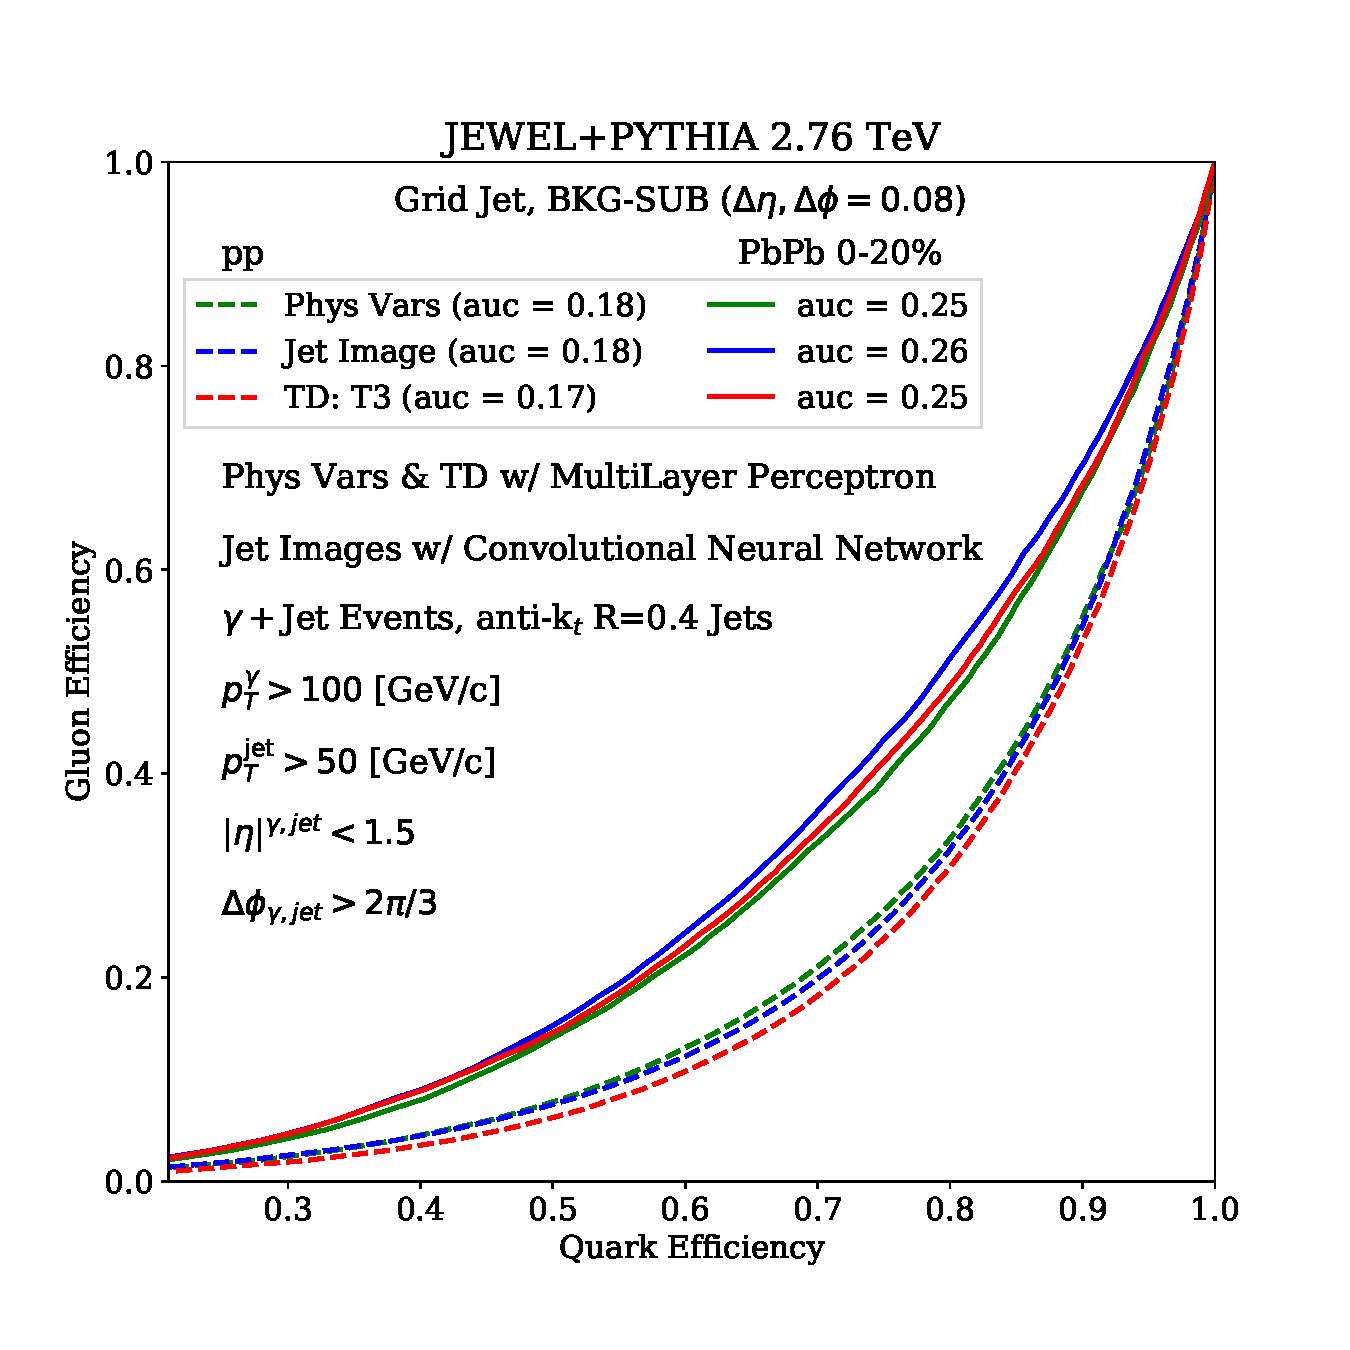
\includegraphics[width=1.0\columnwidth]{Figures/ROC_QvsG_v2.pdf}
	  \label{fig:tjetQCD}
	\end{figure}
	
	\begin{itemize}
	\item All methods suffer losses in classification due to quenching
	\item A quenched quark jets begin to look more like gluon jets 
	\end{itemize}
	

\section{Elucidating medium properties}

	\begin{figure}[t]
	   \centering
	   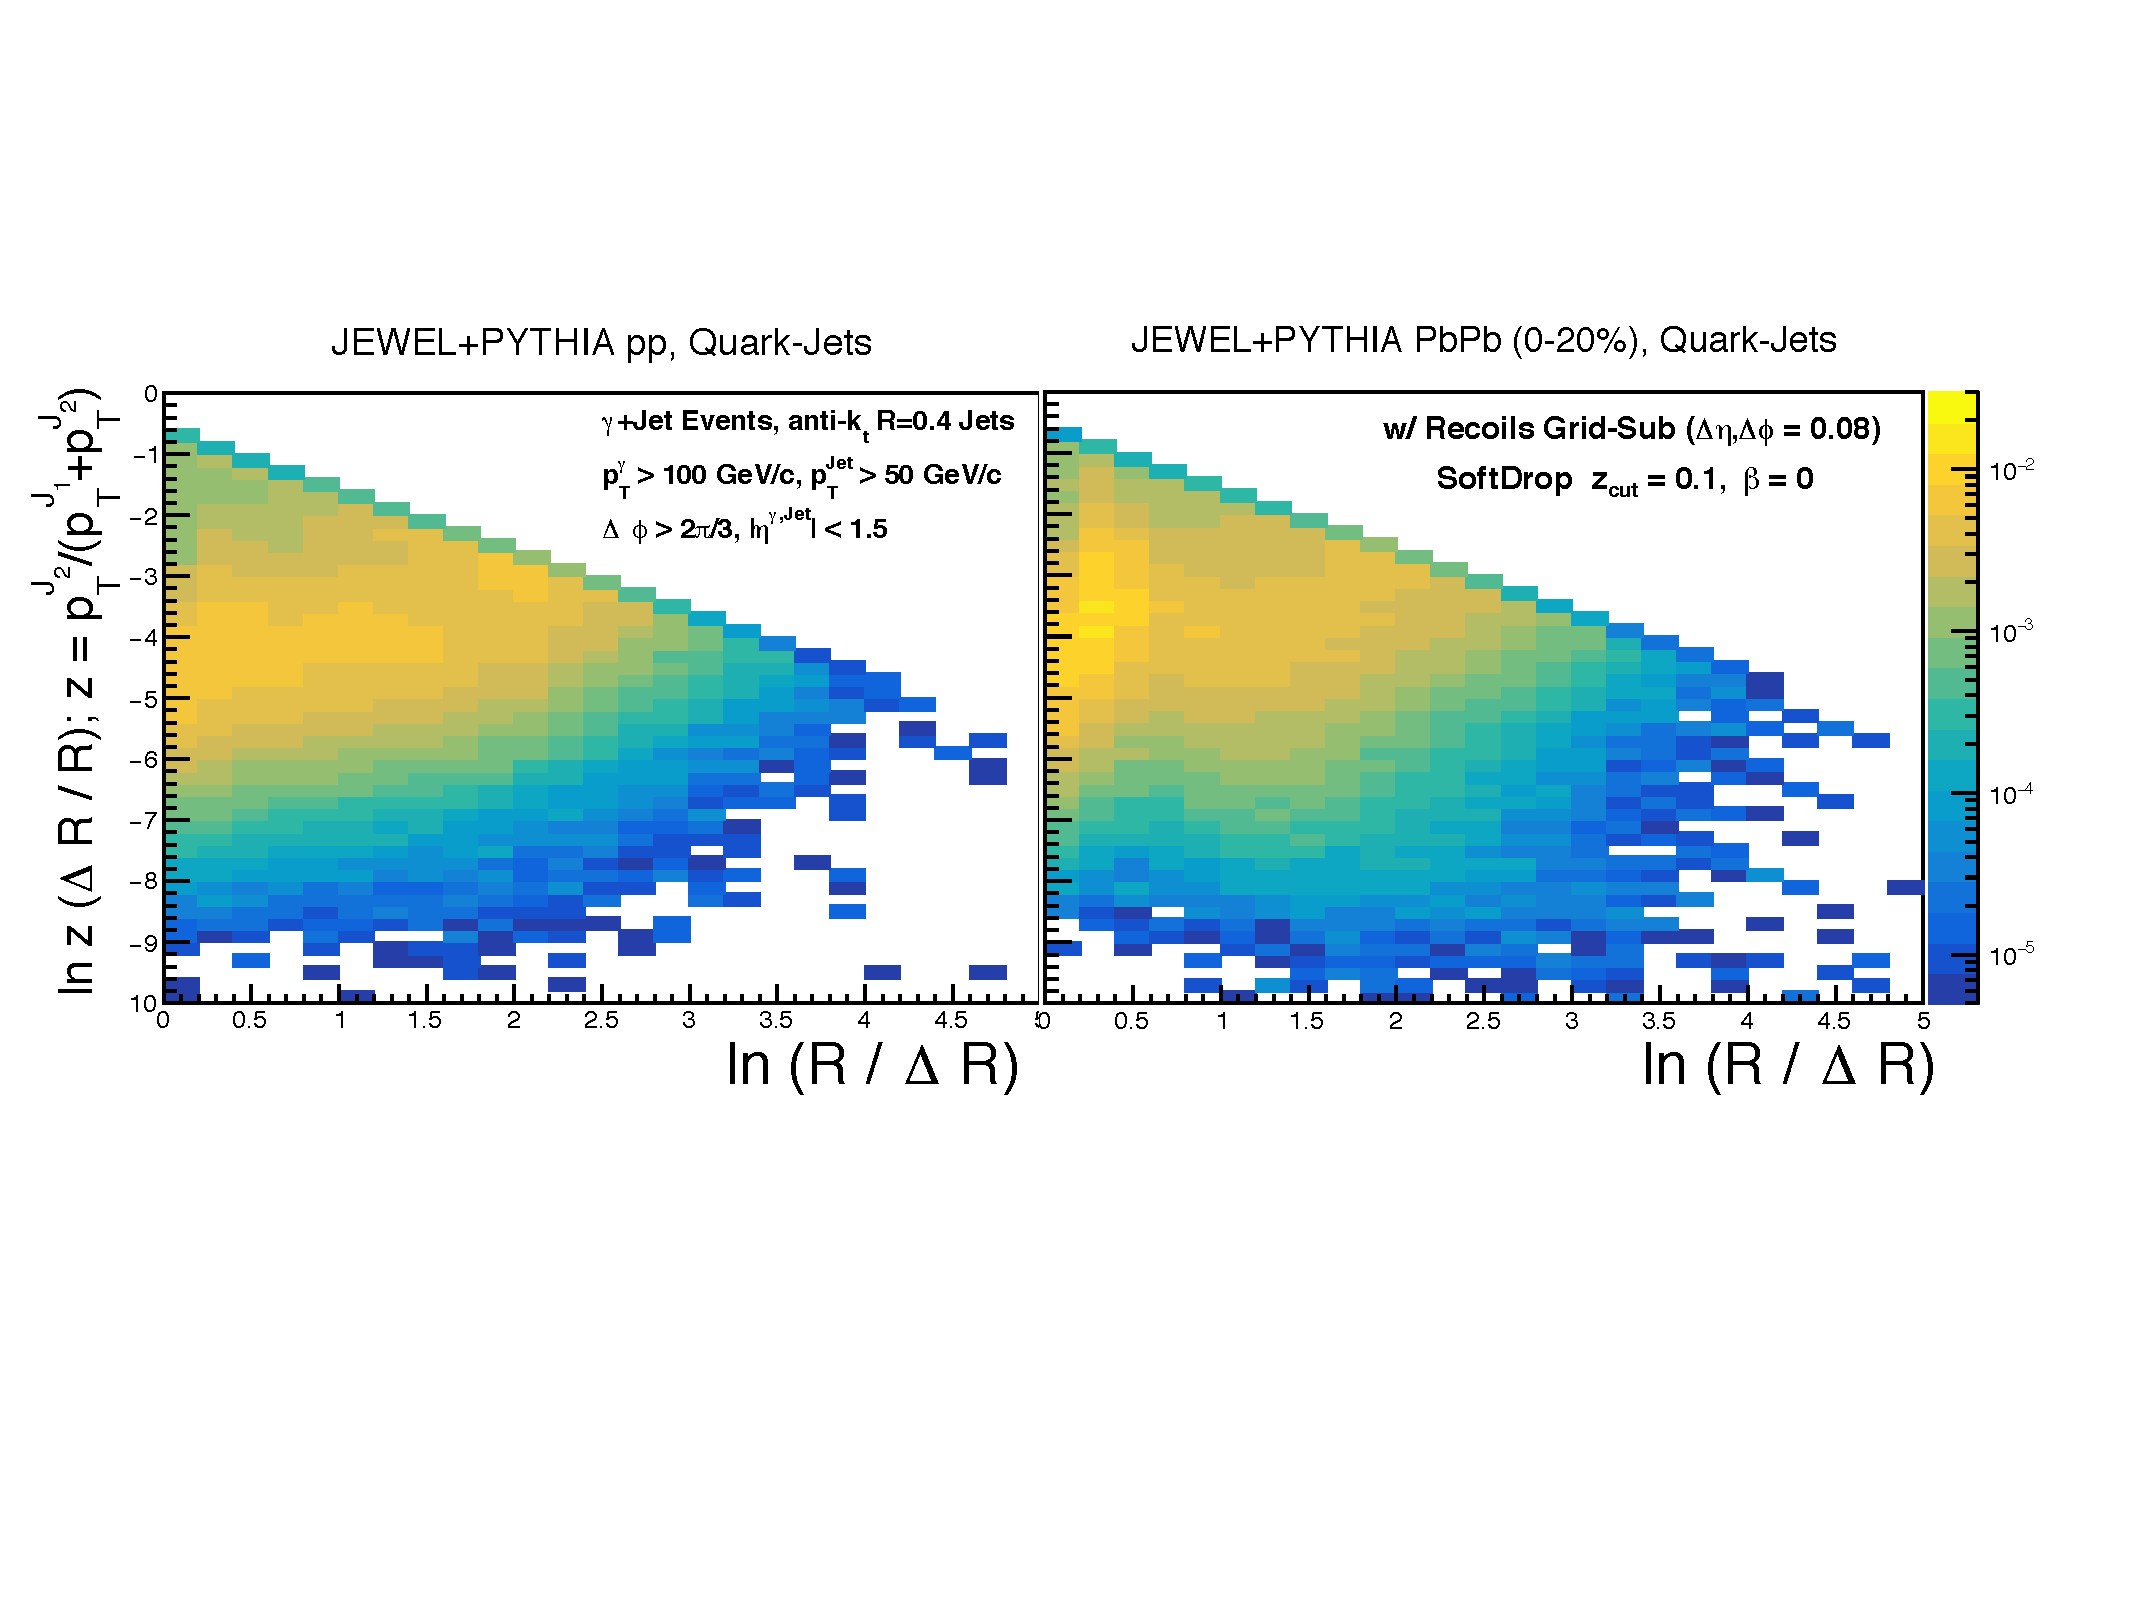
\includegraphics[width=0.9\columnwidth]{Figures/lunddiagram_edit}
	   \label{fig:lunddiagram_qjet}
	\end{figure}

	The Lund diagram is a diagrammatic jet representation associated with the Cambridge/Aachen clustering tree where the the branching kinematics along the hard branches are recorded
	\begin{itemize}
	\item in terms of longitudinal momentum fraction $z$ of the soft branch
	\item the angular separation $\Delta R$ between the two branches
	\end{itemize}

	%For quark jets in vacuum (left) and quenched (right - above), a significantly enhanced region close to the $y$-axis in PbPb collisions that corresponds to increased wide angle, soft radiation in quenched jets. One also sees the modification of jet cores in \jw where subleading subjets tend to have wider angles and softer momenta. These are characteristic features we hope to extract with pure samples of quark and gluon jets, and using the Lund diagram one can directly see the emergence of such qualitative features.

	\subsection{Quantifying effects of jet-grooming}

	\begin{figure}[t]
	   \centering
	   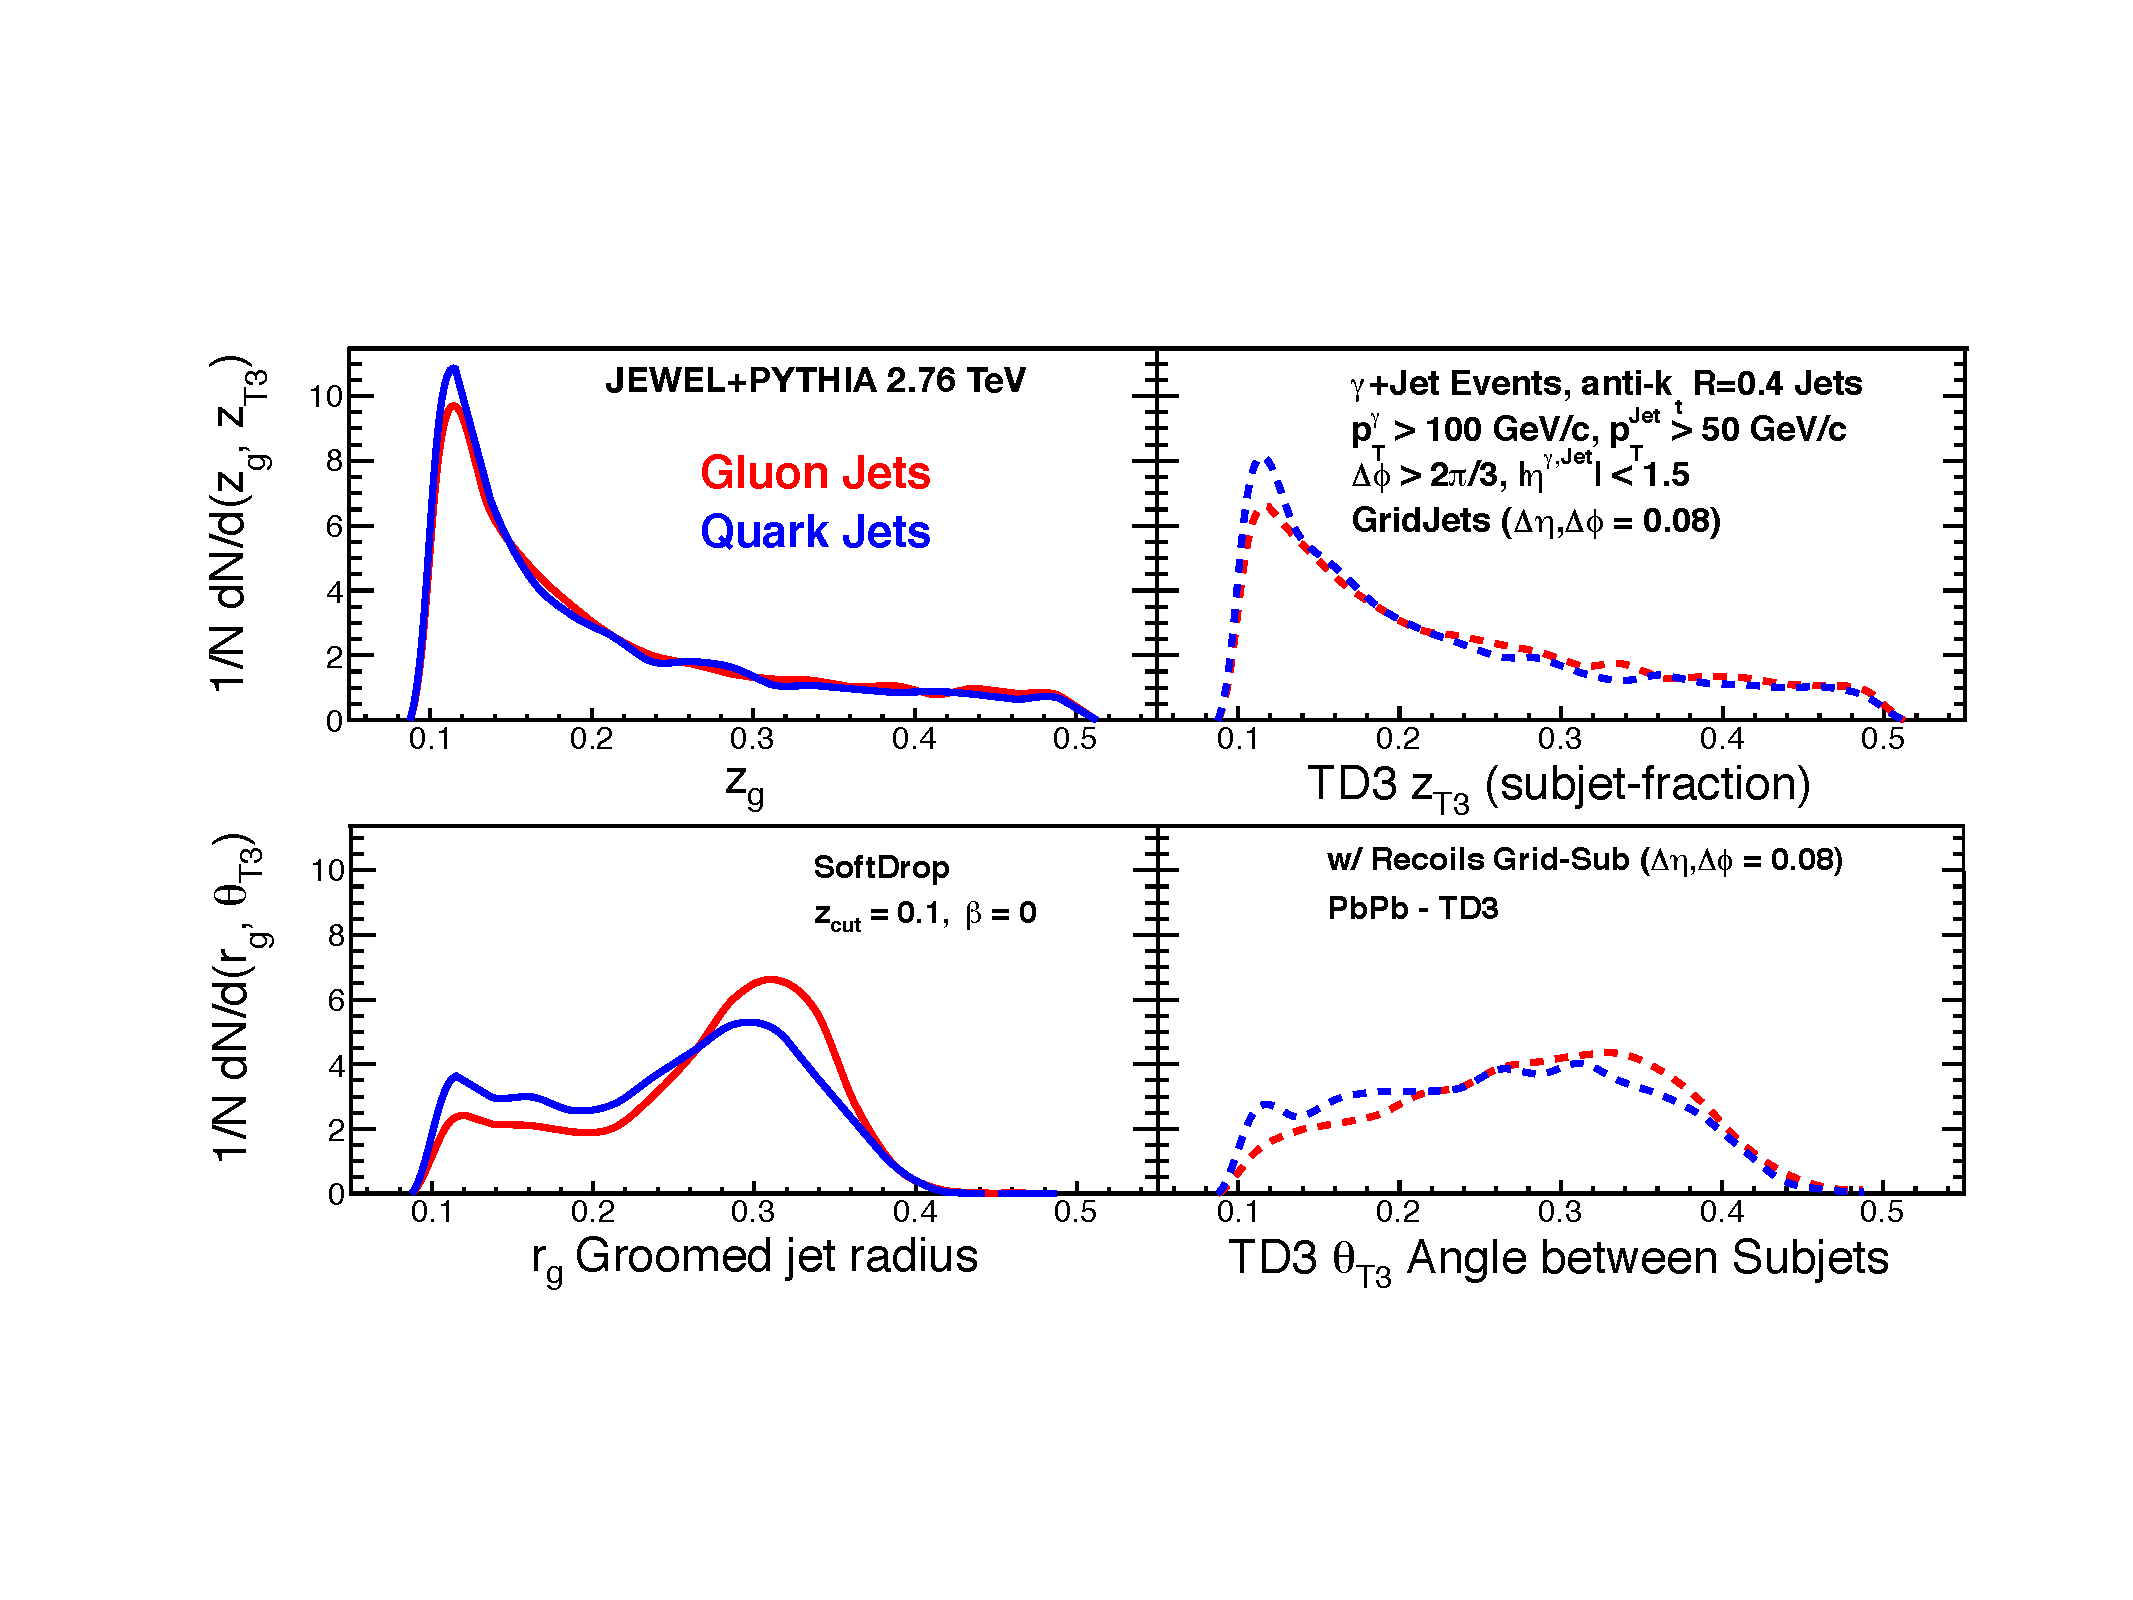
\includegraphics[width=0.9\columnwidth]{Figures/softdrop_vs_td_zgrg}
	   \label{fig:softdrop_zgrg}
	\end{figure}

	Using TD at third order, one can study reproduce effectively physics of the jet shower such as the momentum fraction and angular scale of the first split. 
	\begin{itemize}
	\item SoftDrop removes soft, wide angle radiation from jets
	\item TD reproduces $z$ and showcases a broader $R_{g}$ which is more sensitive to real fragmentation
	\end{itemize}

	We propose to look at the difference between the square of jet mass for ungroomed and soft-drop groomed jets: $\delta m \equiv \sqrt{m_{\rm jet}^2-m_{\rm groomed-jet}^2}$. 
	\begin{figure}[t]
	   \centering
	   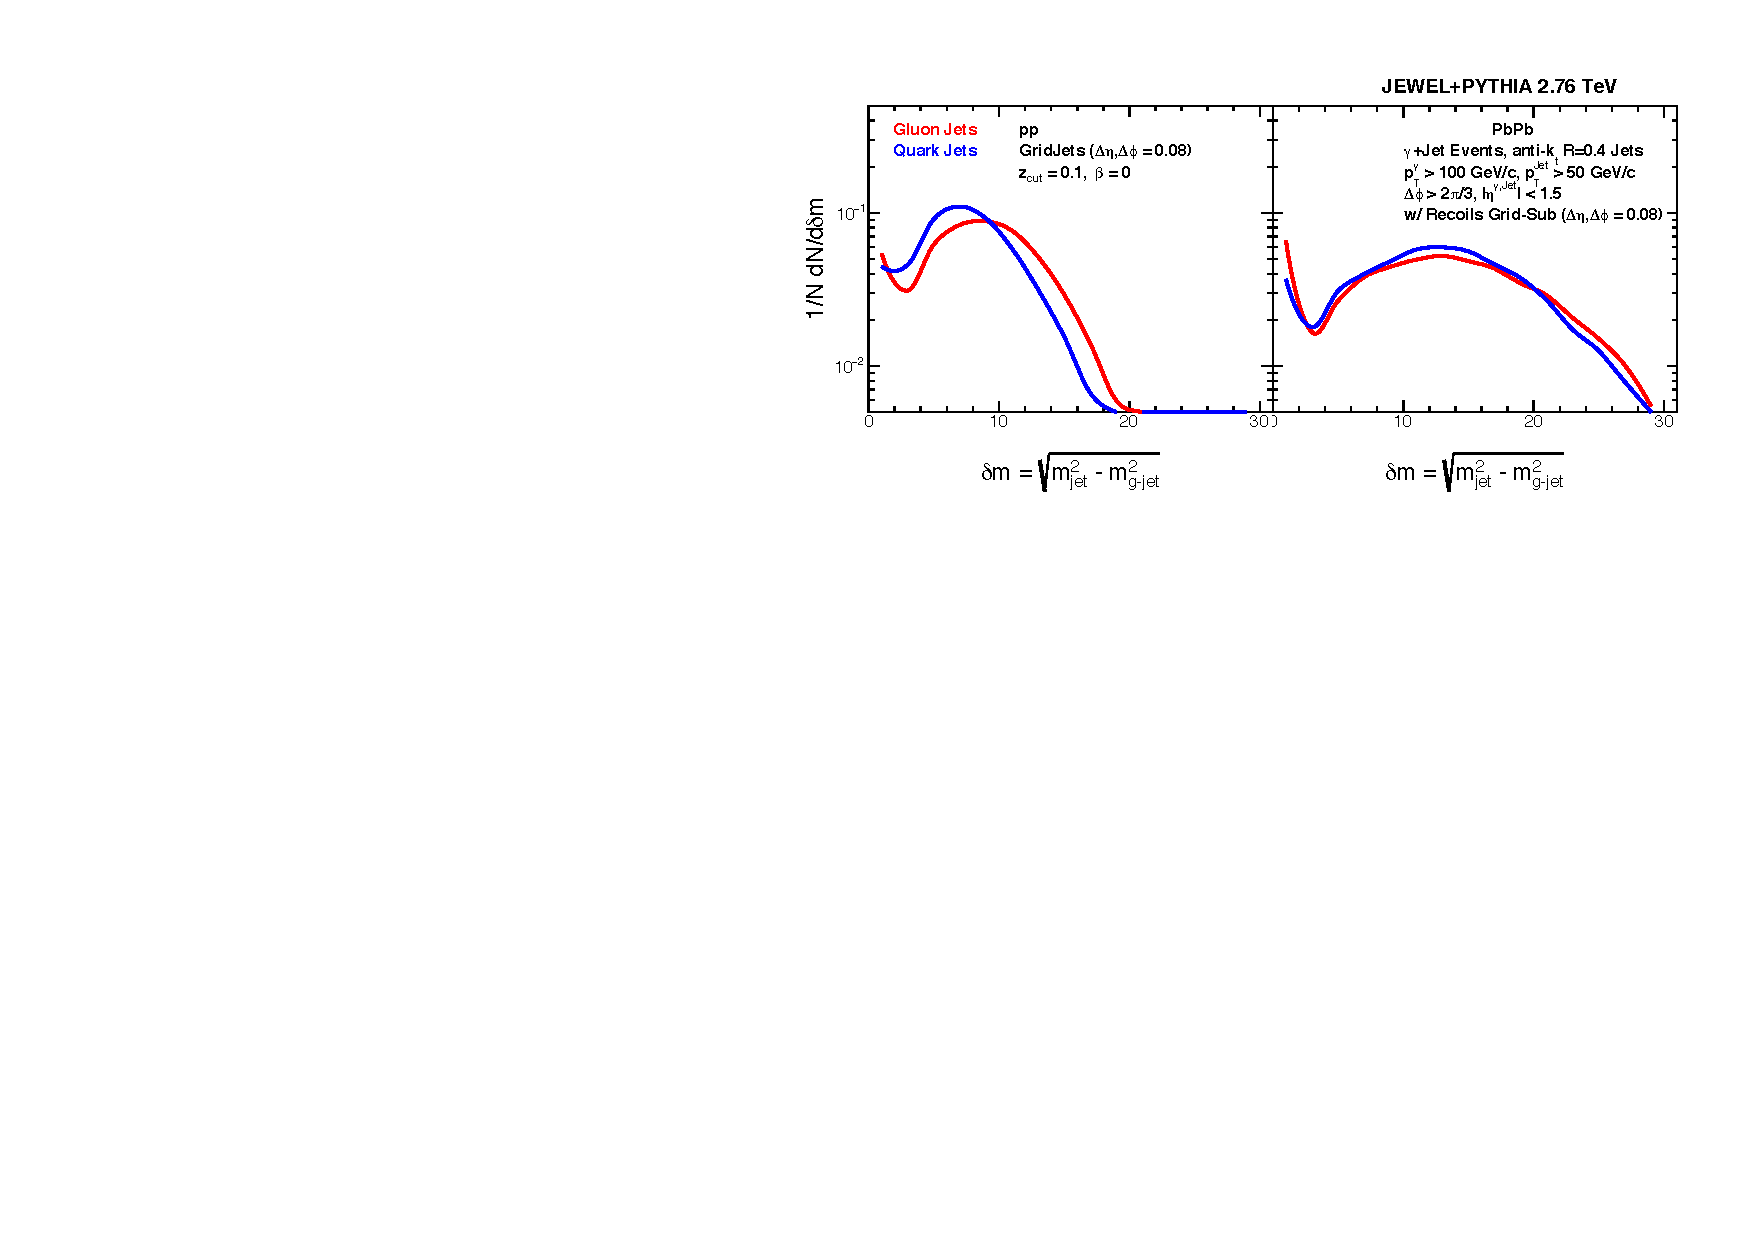
\includegraphics[width=0.9\columnwidth]{Figures/deltaMPrediction.pdf}
	   \label{fig:comp_delta_m2}
	\end{figure}
		
	\begin{itemize}
	\item $\delta m$ disentangles hard, collinear radiation and probes the soft radiation that is dropped. 
	\item vacuum jets exhibits differences between quark and gluon initiated as opposed to quenched jets 
	\item SoftDrop does no mass-grooming for a significant fraction of jets! 
	\end{itemize}
	
\section{Conclusions}
Jet modifications are studied via the novel method of comparing and contrasting the classification of quark jets from gluon jets in different collision systems.
	\begin{itemize}
	\item Q-G classification performance worsens for quenched jets
	\item TD extracts fundamental jet fragmentation patterns 
	\item \jw increase of soft particle multiplicity due to medium recoils throughout the jet region
	\end{itemize}
%In the future, comparisons between theoretical calculations, simulations and experimental measurements will become standard practice in order to identify robust features of jet-medium interactions. Our work represents a thorough, systematic framework that we hope will serve this important purpose.

%All references and further discussion of the ROC curves and jet sub-structure modification in \jw simulations can be found in our paper ``\textit{Probing heavy ion collisions using quark and gluon jet substructure}" arXiv:1803.03589 (Submitted to JHEP). 
	
%==============================================================================
%==End of content==============================================================
%==============================================================================

%--References------------------------------------------------------------------
%\section{References}
%\begin{thebibliography}
%\bibitem{bib1} References here 
%\end{thebibliography}
%--End of references-----------------------------------------------------------

\end{multicols}

%==============================================================================
\end{frame}
\end{document}

